\chapter{Channel Coding}
\label{chapter:ChannelCoding}

\index{channel coding}
\section{Introduction}

\subsection{What is channel coding and why do we use it?}

Channel coding is the art of adding redundancy to a message in order to make it more robust against noise.
It is used because noise and errors are essentially unavoidable in many systems (e.g., wireless communications and magnetic storage).
Coding allows one to trade-off rate for reliability and usually provides large gains in overall system efficiency.
In contrast, source coding (or compression) is used to remove the redundancy from sources (e.g., zip files JPEG pictures).
Channel coding carefully adds redundancy to a message so that it can be transmitted reliably over noisy channels. 

\begin{example}[Repeat Code]
Consider the 1 bit message $u\in\left\{ 0,1\right\} $ mapped to a codeword of length $2t+1$ by repeating the message bit.
This gives a binary code with two codewords:
\[ \mathcal{C}=\{\underbrace{00\ldots00}_{2t+1},\underbrace{11\ldots11}_{2t+1}\}. \]
If fewer than $t$ errors, then received sequence is closer to correct codeword.
Therefore, a decoder which chooses the codeword closest to the received sequence will decode successfully.
For a binary code, the code rate is defined to be
\[R=\frac{\mbox{\# information bits}}{\mbox{\# code bits}},\]
and this gives $\frac{1}{2t+1}$ for the repeat code.
\end{example}


\begin{example}[Credit Card Numbers]
Credit card numbers use a check digit to detect single errors and adjacent transpositions.
Let $\underline{x}$ be a credit card number whose digits are given by $\underline{x}=\left(x_{1},x_{2},\ldots,x_{16}\right)$,
then
\[ \left[\sum_{i=1}^{8}x_{2i}+\sum_{i=1}^{8}\left(2x_{2i-1}\bmod9\right)\right]\bmod10=0\]
Consider the number 5420 1213 7904 9210.
In this case, the first sum gives $4+0+2+3+9+4+2+0=24$ and the second sum gives: $1+4+2+2+5+0+0+2=16$.
So, we have the overall sum $\left[24+16\right]\bmod10=0$.
The code detects single errors because, for $i=1,\ldots,8$, changing $x_{2i}$ to $x_{2i}'$ changes the check value by $x_{2i}'-x_{2i}$ and changing $x_{2i-1}$ to $x_{2i-1}'$ changes the check value by $2(x_{2i}'-x_{2i})\bmod 9$.
Likewise,  swapping $x_{1},x_{2}$ changes the check by
\[ \left[(x_{1}-x_{2})+(2x_{2}\bmod9-2x_{1}\bmod9)\right]\bmod10. \]
\end{example}

Coding is used in many systems and devices including:
\begin{itemize}
\item CD / DVD players : Modulation code + Reed-Solomon (RS) code
\item Digital Video Broadcasting (DVB): Convolutional Code + RS code
\item Deep Space Communications: Advanced Turbo and LDPC codes
\item Cell Phones: Convolutional codes for voice and Turbo/LDPC codes for data
\end{itemize}

\subsection{Channels and Error Models}

\begin{figure}[t]
\begin{center}
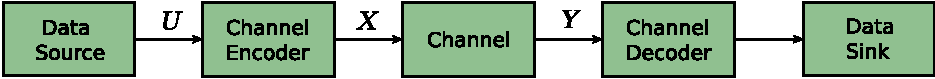
\includegraphics[width=0.95\textwidth,keepaspectratio]{Figures/commfig2}
\end{center}
\vspace{-4mm}
\caption{Block diagram of digital communication from a coding perspective.}
\end{figure}

When designing and analyzing channel codes, one often uses a simple model of a communications channel known as a \defn{channel coding}{discrete memoryless channel} (DMC).
The channel input $X$ is an element of input alphabet $\mathcal{X}$ and the channel output $Y$ is an element of the output alphabet $\mathcal{Y}$.
The main assumption is that each channel use is indepedent and governed by the probability law
\[ W(y|x) \triangleq \Pr\left(Y=y|X=x\right).\]

[Add figure with transition diagrams]

The \defn{channel coding}{binary symmetric channel} (BSC) with error probability $p$ is defined by $\mathcal{X}=\mathcal{Y}=\left\{ 0,1\right\} $ and
\[ W(y|x)=\begin{cases}
p & \mbox{if }x\neq y\\
1-p & \mbox{if }x=y\end{cases}\]
The \defn{channel coding}{binary erasure channel} (BEC) with erasure probability $\epsilon$ is defined by $\mathcal{X}=\left\{ 0,1\right\} $, $\mathcal{Y}=\left\{ 0,1,?\right\}$ and
\[ W(y|x)=\begin{cases}
\epsilon & \mbox{if }y=?\\
1-\epsilon & \mbox{if }x=y\\
0 & \mbox{if }x\neq y\end{cases}\]
The \defn{channel coding}{binary-input AWGN channel} (BIAWGN) with $\sigma^{2}=\frac{N_{0}}{2}$ is defined by $\mathcal{X}=\left\{ -1,1\right\} $, $\mathcal{Y}=\mathbb{R}$ and
\[ W(y|x)=\frac{1}{\sqrt{\pi N_{0}}}e^{-\left|y-x\right|^{2}/N_{0}},\]
where $N_{0}$ is the noise spectral density at the receiver.

The SNR of communication system is defined in terms of the \textbf{energy per information bit},$E_{b}$, and the average \textbf{energy per transmitted symbol}, $E_{s}$.
The conversion between these two quantities is based on keeping track of the units
\[E_{s}=\frac{\mbox{\# information bits}}{\mbox{\# transmitted symbols}}\;\frac{\mbox{Energy}}{\mbox{information bit}}=R'\, E_{b}. \]
The information rate $R'$ (bits/channel use) is equal to the code rate $R$ for binary-input channels.
To make a fair comparisons, one must use the rate-normalized quantity $E_{b}/N_{0}$ (pronounced ebb-no).
The normalization adjusts for the extra energy used to send parity symbols.
The \defn{channel coding}{coding gain} is the reduction in required $E_b / N_0$ to achieve a particular error rate.
In other cases, it more convenient to use the quantity $E_{s}/N_{0}$ (pronounced ess-no).

For example, a bit-error rate (BER) of $10^{-5}$ is achieved by uncoded BPSK transmission with $E_{b}/N_{0}=9.6\;\mathrm{dB}$.
Whereas, a rate-$\frac{1}{2}$ code with moderate decoding complexity (Viterbi decoding of a convolutional code) has a BER of $10^{-5}$ at $E_{b}/N_{0}=4.2\;\mathrm{dB}$.
The coding gain in this case is $9.6-4.2=5.4\;\mathrm{dB}$

\section{The Basics of Coding}

\subsection{Codes}

\begin{figure}[t]
\begin{center}
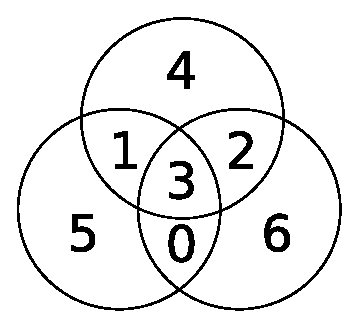
\includegraphics[width=2in,keepaspectratio]{Figures/hammvenn}
\end{center}
\vspace{-4mm}
\caption{Venn diagram representation of the (7,4) binary Hamming code.}
\end{figure}

Let $\mathcal{X}$ be the input alphabet of a channel (assume $\left|\mathcal{X}\right|=q$)
\begin{definition}
A length-$n$ \textbf{code} over the alphabet $\mathcal{X}$ is simply a subset $\mathcal{C}\subseteq\mathcal{X}^{n}$ of all input sequences.
\end{definition}
If a binary code has $M=\left|\mathcal{C}\right|$ codewords, then the code rate is $R=\frac{\log_{2}M}{n}$.
This means we can send $k$ information bits when $M=2^k$.

For example, the binary repeat code of length 5 is defined by $\mathcal{X}=\left\{ 0,1\right\}$ and
\[\mathcal{C}=\left\{ 00000,11111\right\} \subset\left\{ 0,1\right\} ^{5}. \]
Likewise, the binary even parity code of length 3 is
\[ \mathcal{C}=\left\{ 000,110,101,011\right\} \subset\left\{ 0,1\right\} ^{3} . \]

\begin{definition}
The \defn{channel coding}{Hamming distance} $d(\underline{x},\underline{y})$ is equal to the number of places where the vectors differ.
It can be defined mathematically by
\[ d(\underline{x},\underline{y}) = \sum_{i=1}^{n}( 1- \delta_{x_{i},y_{i}}), \]
where $\delta_{a,b}$ is Kronecker delta function
\[\delta_{a,b}=\begin{cases}
0 & \mbox{if }a\neq b\\
1 & \mbox{if }a=b\end{cases}. \]
\end{definition}

The distance between codewords is typically measured with the Hamming distance.
Using this metric, the set $\mathcal{X}^{n}$ forms a discrete metric space
Another important code parameter is the minimum distance $d_{min}$ between any two
codewords is
\[ d_{min}\triangleq\min_{\underline{x},\underline{y}\in\mathcal{C},\underline{x}\neq\underline{y}}d(\underline{x},\underline{y}).\]

\begin{example}[Hamming Code]
The (7,4) binary Hamming Code has $n=7$, $M=16$, and $d_{min}=3$.
The code can be defined in terms of a Venn diagram showing three partially overlapping sets.
Each of the seven subregions represent a code bit and the three circles represent even parity costraints.
Encoding can be done by choosing $x_0,\ldots,x_3$ arbitrarily and then computing the last three parity bits.
Any single error can be corrected by observing each bit error gives a unique pattern of parity violations.
The codewords can be listed as follows:
\[\begin{array}{cccc}
0000000 & 0100110 & 1000011 & 1100101\\
0001111 & 0101001 & 1001100 & 1101010\\
0010101 & 0110011 & 1010110 & 1110000\\
0011010 & 0111100 & 1011001 & 1111111
\end{array} \]
\end{example}

\subsection{Decoding}

Consider the decoding problem for binary codes with $\mathcal{X}=\mathcal{Y}=\left\{ 0,1\right\} $ and $\mathcal{C}\subseteq\mathcal{X}^{n}$.
The channel input is $\underline{x}\in\mathcal{C}$, the received sequence is $\underline{y}$, and the number of errors is $t=d(\underline{x},\underline{y})$
It is not hard to verify that minimum distance decoding, which returns the codeword closest to the channel output, is optimal.
Breaking ties arbitrarily, one can write
\[ \hat{\underline{x}}=\arg\min_{\underline{w}\in\mathcal{C}}d(\underline{w},\underline{y})\]

The following implies that the minimum distance decoder can always correct $t$ errors if $d_{min}\geq2t+1$.
\begin{proposition}
For any received sequence $\underline{y}$, there is at most one codeword $\underline{w}$ such that $d(\underline{y},\underline{w})\leq\frac{d_{min}-1}{2}$.
\end{proposition}
\begin{proof}
Suppose there are codewords $\underline{w},\underline{z}$ where $d(\underline{y},\underline{w})$ and $d(\underline{y},\underline{z})$
are $\leq\frac{d_{min}-1}{2}$.
Then, the triangle inequality implies $d(\underline{w},\underline{z})\!\leq\! d(\underline{y},\underline{w})\!+\! d(\underline{y},\underline{z})\!\leq\! d_{min}-1$ and contradicts the definition of $d_{min}$.
Therefore, if $t\leq\frac{d_{min}-1}{2}$, then $\underline{x}$ is the unique codeword such that $d(\underline{x},\underline{y})\leq\frac{d_{min}-1}{2}$.
\end{proof}

The following allows simultaneous error correction of $t$ errors and detection of $d$ errors.
\begin{proposition}
If $d_{min}\geq t+d+1$ and $d\geq t$, then a single decoder can
both correct $t$ and detect $d$ errors.
\end{proposition}
\begin{proof}
Assume that each codeword is surrounded a inner ball of radius $t$ and an outer ball of radius $d$.
If the received vector is in an inner ball, decode to the codeword at the center.
Otherwise, declare decoding failure.

From the previous result, we see that no two inner balls overlap and that the inner ball of one codeword does not overlap the outer ball of any codeword.
If the number of errors is at most $t$, then received vector will be in the inner ball of the transmitted codeword and will be decoded correctly.
If the number of errors is between $t+1$ and $d$, then received vector will not be in the inner ball of any codeword and failure will be declared.
\end{proof}

\begin{proposition}
If $d_{min}\geq e+1$, then there is a decoder which corrects all patterns of $e$ erasures.
\end{proposition}
\begin{proof}
Make a list of all codewords and then erase any $e$ positions.
Each erasure reduces the minimum distance between any two codewords by at most one.
After $e$ steps, the new $d_{min}\geq e+1-e=1$.
This implies that the codewords, defined by the remaining symbols, are all unique.
\end{proof}

\section{Binary Linear Codes}


\subsection{Basic Properties}

\begin{table}
\begin{center}
\begin{tabular}{c||c|c}
+ & 0 & 1\tabularnewline
\hline
\hline
0 & 0 & 1\tabularnewline
\hline 
1 & 1 & 0\tabularnewline
\end{tabular}~~~\begin{tabular}{c||c|c}
{*} & 0 & 1\tabularnewline
\hline
\hline
0 & 0 & 0\tabularnewline
\hline 
1 & 0 & 1\tabularnewline
\end{tabular}
\caption{The addition and multiplication operations for the binary field.}
\label{tab:BinaryField}
\end{center}
\end{table}

This chapter focuses almost exclusively on binary linear codes, which are the simplest and most important class of error-correcting codes.
The restriction to linear codes can be motivated by two things: simplicity and performance.
We will see later that linear codes are much simpler to describe, encode, and analyze.
Moreover, there are very few cases where non-linear codes are better than linear codes.
So, there is essentially no performance penalty for this simplicity.

Linear codes, like linear algebra, make use of matrices and vectors of elements that can be added, subtracted, multipled, and divided.
A set of numbers which obey all the standard rules of arithmetic is an algebraic object known as a \textbf{field}.
For example, the real and complex numbers are both fields.

There are also fields which have a finite number of elements.
Let $a,d$ be positive integers so that the division of $a$ by $d$ gives the equation $a = dq+r$, where $q$ is quotient and $0\leq r \leq d-1$ is the remainder.
The modulo operation is defined to return the remainder from division and is denoted $r = a \bmod d$.
It turns out that the binary alphabet, $\left\{ 0,1\right\} $, with standard arithmetic ($+,-,*,/$) performed modulo 2 is also a field.
The operations are shown explicitly in Table~\ref{tab:BinaryField}.

For linear algebra over a field, the scalar (i.e., field) operations are used to define vector and matrix operations.
Vector addition is defined element-wise, so that $\left[\underline{x}+\underline{y}\right]_{i}=x_{i}+y_{i}$.
An $(n,k)$ \defn{channel coding}{binary linear code} is $\mathcal{C}\subseteq\left\{ 0,1\right\} ^{n}$ with $\left|\mathcal{C}\right|=2^{k}$ where $\underline{x},\underline{y}\in\mathcal{C}$ implies $\underline{x}+\underline{y}\in\mathcal{C}$
Since $\underline{x}+\underline{x}=\underline{0}$, this implies all zero vector $\underline{0}\in\mathcal{C}$.
For example, the $n=3$ ``even parity'' code is a (3,2) binary linear code with codewords $\mathcal{C}=\left\{ 000,110,101,011\right\} $.

\begin{definition}
The \defn{channel coding}{Hamming weight} $w(\underline{x})$ is the number of non-zero elements in $\underline{x}$ or
\[ w(\underline{x}) = \sum_{i=1}^{n}(1-\delta_{x_i , 0}). \]
For binary vectors, this also implies that the Hamming distance is given by
\[d(\underline{x},\underline{y})=w(\underline{x}-\underline{y}). \]
\end{definition}

Linear codes also have a simplified distance structure.
Instead of considering the minimum distance between all codewords, it suffices to focus only on the all-zero codeword.

\begin{proposition}
The minimum distance of a linear code is given by
\[ d_{min} =\min_{\underline{x}\in\mathcal{C},\underline{x}\neq\underline{0}}w(\underline{x}-\underline{y}). \]
\end{proposition}
\begin{proof}
The linear property of the code allows one to translate computations involving the distance between two codewords to expressions involving the Hamming weight of one codeword.
This gives
\begin{align*}
d_{min}
&\triangleq\min_{\underline{x},\underline{y}\in\mathcal{C},\underline{x}\neq\underline{y}}d(\underline{x},\underline{y}) \\
&=\min_{\underline{x},\underline{y}\in\mathcal{C},\underline{x}\neq\underline{y}}w(\underline{x}-\underline{y}) \\
&=\min_{\underline{x}\in\mathcal{C},\underline{x}\neq\underline{0}}w(\underline{x}-\underline{y}),
\end{align*}
where the last step follows from the fact that
\[ \left\{\underline{x}-\underline{y} \,|\, \underline{x},\underline{y}\in\mathcal{C},\underline{x}\neq \underline{y} \right\}
= \left\{\underline{x}\in\mathcal{C} \,|\, \underline{x}\neq \underline{0} \right\}. \]
\end{proof}

\subsection{Generator and Parity-Check Matrices}

Linear codes can be represented compactly using matrices.
The generator defines the code by allowing one to list all the codewords.

\begin{definition}
The \defn{channel coding}{generator matrix} $\underline{G}$ of an $(n,k)$ binary linear code is a $k\times n$ binary matrix such that all codewords, $\underline{x}\in\mathcal{C}$, can be written as $\underline{u}\cdot\underline{G}=\underline{x}$ for some message vector $\underline{u}\in\left\{ 0,1\right\} ^{k}$.
Therefore, the code is the row space of $\underline{G}$).
\end{definition}

\begin{example}
The generator matrix
\[\underline{G}=\left[\begin{array}{ccccc}
1 & 0 & 1 & 1 & 0\\
1 & 1 & 1 & 0 & 1\end{array}\right] \]
defines the $(5,2)$ code
\[ \mathcal{C} = \left\{ 00000,10110,01011,11101\right\}. \]
Encoding $\underline{u}=[11]$ gives $\underline{u}\cdot\underline{G}=[0\,\,1\,\,0\,\,1\,\,1]$
\end{example}

If $\underline{G}$ has full rank $k$ (over the binary field), then the code has $2^{k}$ distinct codewords.
Otherwise, some non-zero messages encode to the all-zero codeword and there are at most $2^{k-1}$ codewords.

\begin{definition}
The generator matrix is in \defn{channel coding}{systematic form} if $\underline{G}=\left[\underline{P}\,\,\,\underline{I}_{k}\right]$, where $\underline{I}_{k}$ is the $k\times k$ identity matrix.
The matrix $\underline{P}$ is called the \defn{channel coding}{parity generator} of the code because $\underline{u}\cdot\underline{P}$ computes the parity bits for $\underline{u}$.
For a generator matrix in systematic form, the message vector appears in codeword
\[\underline{u}\cdot\underline{G}=\underline{u}\cdot\left[\underline{P}\;\;\underline{I}_{k}\right]=\left[\underline{u}\!\cdot\!\underline{P}\;\;\underline{u}\right]. \]
\end{definition}

The parity-check (PC) matrix defines the code by listing the parity-check equations that each codeword must satisfy.

\begin{definition}
The \defn{channel coding}{parity-check matrix} $\underline{H}$ of an $(n,k)$ binary linear code is an $(n-k)\times n$ binary matrix such that $\underline{x}\cdot\underline{H}^{T}=\underline{0}$ for all $\underline{x}\in\mathcal{C}$.
Therefore, the code is the null space of $\underline{H}$.
\end{definition}

While the generator matrix defines the code and an encoder, the parity-check matrix defines only the code; there is no implied encoder.
There is also a relationship between and generator and parity-check matrix for the same code.
Recall that, for all codewords $\underline{x}$,  there is a message $\underline{u}$ such that $\underline{x}=\underline{u}\cdot\underline{G}$.
This means that $\underline{G}\cdot\underline{H}^{T}=\underline{0}$.

\begin{example}
For the $(5,2)$ code we saw previously, one possible parity-check matrix is
\[ \underline{H}=\left[\begin{array}{ccccc}
1 & 0 & 0 & 1 & 1\\
0 & 1 & 0 & 0 & 1\\
0 & 0 & 1 & 1 & 1\end{array}\right]. \]
Notice that it satisfies $\underline{G}\cdot\underline{H}^{T}=0$ for the previous $\underline{G}$.
\end{example}

In general, we assume that $\underline{H}$ has full rank.
Otherwise, there are redundant constraints and some row can eliminated without changing the code.

A parity-check matrix is in \defn{channel coding}{systematic form} if $H=\left[\underline{I}_{n-k}\,\,\,\,-\underline{P}^{T}\right]$.
When both the generator and parity-check matrices are in systematic form, we can write
\begin{align*}
\underline{G}\cdot\underline{H}^{T}
&=\left[\underline{P}\,\,\,\,\underline{I}_{k}\right]\cdot\left[\underline{I}_{n-k}\,\,\,\,-\underline{P}^{T}\right]^{T} \\
&=\left[\underline{P}\,\,\,\,\underline{I}_{k}\right]\cdot \left[ \begin{array}{c} \underline{I}_{n-k} \\ -\underline{P} \end{array} \right] \\
&=\underline{P}-\underline{P} \\
&=\underline{0}.
\end{align*}

\begin{example}
A \textbf{single parity-check code} is an $(n,n-1)$ binary linear code with parity-check matrix
\[ H=[\underbrace{1,1,\ldots,1}_{n\;\mathrm{times}}]. \]
For all codewords $\underline{x}$, the parity-check constraint $\underline{x}\cdot\underline{H}^{T}=\underline{0}$ implies that $\sum_{i=1}^{n}x_{i}\bmod2=0$ (i.e., the codeword has an even number of ones).
The minimum distance is $d_{min} = 2$ and the generator matrix is given by
\begin{equation*}
G=\left[\begin{array}{ccccc} 1 & 1 & 0 & \cdots & 0 \\ 1 & 0 & 1 & \cdots & 0 \\ \vdots & 0 & \ldots & \ddots & 0 \\ 1 & 0 & 0 & 0 & 1 \end{array}\right].
\end{equation*}
\end{example}

Next, we consider the minimum distance of a code in terms of its generator and parity check matrices.
In general, it is very difficult to compute the minimum distance without enumerating all codewords.
But, one can get upper and lower bounds on the minimum distance much more easily.
In this way, the minimum distance can be found approximately.

Since the minimum distance is equal to the minimum of the Hamming weight overall codewords, it is clearly upper bounded by the Hamming weight of any particular non-zero codeword.
This gives, for any non-zero codewords $\underline{x}$,
\[ d_{min} \leq w(\underline{x}). \]
Likewise, the parity-check matrix can be used to lower bound the minimum distance.
\begin{proposition}
The minimum distance of a code with parity-check matrix
\[\underline{H}=\left[\underline{h}_{1},\underline{h}_{2},\ldots,\underline{h}_{n}\right] \]
is equal to the minimum number of columns that sum to zero or
\[ d_{min}=\min\left\{ w(\underline{x})|\underline{x}\cdot\underline{H}^{T}=\underline{0},\underline{x}\in\left\{ 0,1\right\} ^{n}\backslash\underline{0}\right\}. \]
\end{proposition}
\begin{proof}
Notice that
\[ \underline{x}\cdot\underline{H}^{T}=\sum_{i=1}^n x_{i}\underline{h}_{i}=\sum_{i:x_{i}=1}\underline{h}_{i}, \]
where $\underline{h}_{i}$is the $i$th column of $\underline{H}$.
Therefore, the statement that $\underline{x}\cdot\underline{H}^{T}=\underline{0}$ (i.e., $\underline{x}$ is a codeword) is equivalent to the statement that the sum of $w(\underline{x})$ columns is $\underline{0}$.
Taking the minimum over all non-zero codewords gives the minimum distance.
\end{proof}

One can also bound the minimum distance in terms of error-correction ability.
Recall that a code corrects all error patterns of weight $t$ if and only if $d_{min}\geq2t+1$.
This gives a simple lower bound on the minimum distance.

\begin{example}
Correcting all single errors requires $\frac{d_{min}-1}{2}=1$ or $d_{min}=3$.
Let us try to find the longest code, for a fixed number of parity bits $m$, that corrects all single errors.
In this case, $\underline{H}$ is  matrix with $m$ rows and we can add columns, one at a time, until it is not possible to add a column without losing the ability to correct a single error.
How many columns can we choose?
The maximum value is $n=2^m -1$ and the resuting optimal code is called the binary \defn{channel coding}{Hamming code} of length $n$.
\end{example}

\subsection{Decoding}

Assume a codeword $\underline{x}\in\mathcal{C}$ is transmitted over a channel and $\underline{r}=\underline{x}+\underline{e}$ is received, where $\underline{e}$ is the \textbf{error pattern} with $w(\underline{e})$ errors.
For any received sequence $\underline{r}$, a \textbf{decoder} either returns a codeword $\underline{\hat{x}}=D(\underline{r})$ or declares failure.
The decoded message $\underline{\hat{u}}$ associated with $\underline{\hat{x}}$ is the unique message satisfying $\underline{\hat{x}} = \underline{\hat{u}} \underline{G}$.
A decoder makes
\begin{itemize}
\item a \textbf{block error} (or word error) if $\underline{\hat{x}}\neq\underline{x}$ and $P_{B}$ is used to denote the probability of block error,
\item $b$ \textbf{code bit errors} if $w(\underline{\hat{x}}-\underline{x})=b$ and $P_{b}$ is used to denote the probability that a randomly chosen bit in $\underline{\hat{x}}$ is in error,
\item and $b$ \textbf{message bit errors} if $w(\underline{\hat{u}}-\underline{u})=b$ and $P_{b}$ is used to denote the probability that a randomly chosen bit in $\underline{\hat{u}}$ is in error.
\end{itemize}
From this, we see that the probability of bit error $P_{b}$ can have multiple meanings.
The correct meaning can usually be inferred from the context.
Decoding can also be simplified for linear codes.

\begin{definition}
Let $\underline{s}=\underline{r}\cdot\underline{H}^{T}$ be the \textbf{syndrome} of the received vector $\underline{r}$.
\end{definition}
It turns out that $\underline{s}$ depends only on the error pattern.
Since $\underline{x}\in\mathcal{C}$, we have
\[ \underline{s}=\underline{r}\cdot\underline{H}^{T}=(\underline{x}+\underline{e})\cdot\underline{H}^{T}=\underline{x}\cdot\underline{H}^{T}+\underline{e}\cdot\underline{H}^{T}=\underline{e}\cdot\underline{H}^{T}. \]

A \defn{channel coding}{syndrome decoder} $\underline{\hat{e}}=D_{s}(\underline{s})$ maps the syndrome $\underline{s}$ to an estimated error pattern $\underline{\hat{e}}$.
Let us define the equivalence relation $\sim$ by $\underline{x}\sim\underline{y}$ iff $\underline{x}\cdot\underline{H}^{T}=\underline{y}\cdot\underline{H}^{T}$.
This means that two binary vectors are equivalent if they have the same syndrome.
A syndrome decoder can be designed correct exactly one error pattern in each equivalence class.
The best choice for correction is the most-likely error pattern in that equivalence class.
For most channels, these vectors are chosen to be the minimum weight vector in the equivalence class.

The \defn{channel coding}{standard array} is way of listing all vectors of length-$n$ that exposes the connectiion between syndromes, codewords, and error correction.
In general, it is a $2^{n-k}\times 2^k$ table that contains each length-$n$ binary vector exactly once.
The main idea behind this table is that, when one chooses to correct a particular error pattern, the decoder is automatically defined for all received sequences equal to that error pattern plus a codeword.
Of course, this limits one's ability choose correctable error patterns.


Each row is indexed by a syndrome $\underline{s}$ and contains all binary vectors $\underline{x}$ that satisfy the equation $\underline{s}=\underline{x}\cdot\underline{H}^{T}$.
The first row is reserved for $\underline{s}=\underline{0}$ and contains the all-zero codeword $\underline{c}_1$ in the first column followed the remaining codewords $\underline{c}_2,\ldots,\underline{c}_{2^k}$ in any order.
The first column contains the correctable error patterns $\underline{e}_1 ,\ldots, \underline{e}_{2^{n-k}}$ where $\underline{e}_1$ is the all-zero sequence.
The row-$i$ column-$j$ entry always contains $\underline{e}_i + \underline{c}_j$, and is therefore defined by the first row and first column of the table.
The column associated with a particular codeword can be seen as all the received vectors that will be decoded to that codeword.


Using the parity-check matrix for our $(5,2)$ our example code, the process is as follows
\begin{enumerate}
\item Start with 8 by 5 table and list the zero syndrome and all codewords on first row
\item Pick a minimum weight vector of length $n$ that is not already in table and compute its syndrome
\item Add a new row by writing syndrome followed by the minimum weight vector plus each codeword
\item Repeat from step 2 until table is complete.
\end{enumerate}
The resulting standard array is
\begin{center}
\begin{tabular}{|c||c|c|c|c|}
\hline 
syn\textbackslash cw &  00000 & 10110 & 01011 & 11101\tabularnewline
\hline
\hline 
100 & 10000 & 00110 &  & 01101\tabularnewline
\hline 
010 & 01000 &  & 00011 & \tabularnewline
\hline 
001 & 00100 & 10010 &  & 11001\tabularnewline
\hline 
101 & 00010 &  & 01001 & \tabularnewline
\hline 
111 & 00001 & 10111 &  & 11100\tabularnewline
\hline 
110 & 11000 & 01110 & 10011 & \tabularnewline
\hline 
011 & 01100 & 11010 &  & 10001\tabularnewline
\hline
\end{tabular}
\end{center}
To see if you understand this example, try filling in the missing entries.
One can prove that this process always enumerates all $2^{n}$ binary vectors, so you can test your answers by checking if all binary vectors appear in the table exactly once.

\begin{example}
To see syndrome decoding in action, let $\underline{x}=10110$ and $\underline{e}=11000$.
Then, $\underline{r}=01110$ and $\underline{s}=110$.
Looking in the syndrome table, we find that $\underline{\hat{e}}=11000$ and $\underline{\hat{x}}=10110$.
\end{example}

\subsection{Manipulating Linear Codes}

It follows from linear algebra that any $\underline{G},\underline{H}$ can be put in systematic form using elementary row operations and (possibly) a column permutation.
For the parity-check matrix $H$, the basic idea is to use elemtary row operations to form an identity matrix in the first few columns (i.e., put it in reduced row-echelon form).
For the generator matrix $G$, elementary row operations are used to form an identity matrix in the last few columns.
Sometimes an identity cannot be formed in the desired columns and a column permutation is required to complete the process.
For this reason, two codes are called \textbf{equivalent} if and only if they differ only in the order of the code symbols.

\begin{definition}
For a matrix, an \textbf{elementary row operation} is any one of the following operations:
\begin{enumerate}
\item interchaging any two rows,
\item scaling any row by a non-zero constant,
\item and adding a multiple of one row to another row.
\end{enumerate}
\end{definition}

\begin{example}
In this example, we consider a parity-check matrix
\[ \underline{H} =\left[\begin{array}{cccccc}
1 & 1 & 0 & 1 & 0 & 0\\
0 & 1 & 1 & 0 & 1 & 0\\
1 & 1 & 0 & 0 & 1 & 1\end{array}\right] \]
that requires a column permutation for systematic form.
Let us put $\underline{H}$ is reduced row-echelon form and then find a column permutation to achieve an identity in the first few rows.
The first step gives
\[ \underline{H} \rightarrow\left[\begin{array}{cccccc}
1 & 1 & 0 & 1 & 0 & 0\\
0 & 1 & 1 & 0 & 1 & 0\\
0 & 0 & 0 & 1 & 1 & 1\end{array}\right]\rightarrow\left[\begin{array}{cccccc}
1 & 0 & 1 & 1 & 1 & 0\\
0 & 1 & 1 & 0 & 1 & 0\\
0 & 0 & 0 & 1 & 1 & 1\end{array}\right]
\rightarrow\left[\begin{array}{cccccc}
1 & 0 & 1 & 0 & 0 & 1\\
0 & 1 & 1 & 0 & 1 & 0\\
0 & 0 & 0 & 1 & 1 & 1\end{array}\right], \]
and a column permutation gives
\[ \tilde{\underline{H}}=\left[\begin{array}{cccccc}
1 & 0 & 0 & 1 & 0 & 1\\
0 & 1 & 0 & 1 & 1 & 0\\
0 & 0 & 1 & 0 & 1 & 1\end{array}\right]. \]
Now, we can compute parity generator and generator associated with $\tilde{\underline{H}}$ to get
\[ \tilde{\underline{P}}=\left[\begin{array}{ccc}
1 & 1 & 0\\
0 & 1 & 1\\
1 & 0 & 1\end{array}\right] \quad 
\tilde{\underline{G}}=\left[\begin{array}{cccccc}
1 & 1 & 0 & 1 & 0 & 0\\
0 & 1 & 1 & 0 & 1 & 0\\
1 & 0 & 1 & 0 & 0 & 1\end{array}\right]. \]
Finally, reversing the column permutation gives, for the original code, a generator
\[\underline{G}=\left[\begin{array}{cccccc}
1 & 1 & 1 & 0 & 0 & 0\\
0 & 1 & 0 & 1 & 1 & 0\\
1 & 0 & 0 & 1 & 0 & 1\end{array}\right]  \]
that contains an identity in a subset of its columns.
\end{example}

\section{Performance Analysis}

Consider an $(n,k)$ binary code of rate $R=k/n$ with $d_{min} \geq 2t^* + 1$ and a decoder that corrects all error patterns of weight at most $t^*$.
It is relatively easy to upper bound the probability of block error when this code and decoder are used on a BSC, because a block error cannot occur unless there are more than $t^*$ errors.
This gives
\[ P_{B}\leq1-\sum_{i=0}^{t^*}{n \choose i}p^{i}(1-p)^{n-i}=\sum_{i=t^*+1}^{n}{n \choose i}p^{i}(1-p)^{n-i}. \]
If $p$ is small enough, then we can approximate this by the first term in the sum
\[ P_{B} \approx {n \choose t^* + 1}p^{t^* + 1}.\]
If the code bits are transmitted over an AWGN channel using BPSK followed by a hard-decision detector, then we also have
\[ p= Q\left( \sqrt{\frac{2 E_s}{N_0}} \right) = Q\left( \sqrt{\frac{2 R  E_b}{N_0}} \right). \]
The latter expression allows us to make relatively fair comparisons between coding systems with different rates.
 
\begin{definition}
The \defn{channel coding}{coding gain} achieved by a channel code is the reduction in $E_b / N_0$ required achieve a particular error rate.
For example, if the uncoded system achieves an error rate of $10^{-5}$ at $E_b / N_0 = 9.6$ dB and the coded system achieves an error rate of $10^{-5}$ at $E_b / N_0 = 6.6 dB$, then the coding gain is $9.6 - 6.6 = 3$ dB at the error rate $10^{-5}$.
The coding gain often approaches a limit, for low error rates, known as the \textbf{asymptotic coding gain}.
\end{definition}

Now, we compute the asymptotic coding gain, in terms of $t^*$ and $R$, of hard-decision decoding of a block code.
For the uncoded system, let $\gamma_u$ be the $E_b / N_0$ so that the probability of block error is given by
\[ P_{B}^{(u)}(\gamma_u) = 1- \left(1 - Q\left( \sqrt{2 \gamma_u} \right) \right)^k. \]
For the coded system, let $\gamma_c$ be the $E_b / N_0$ so that the probability of block error is
\[ P_{B}^{(c)}(\gamma_c) \approx {n \choose t^* + 1} Q\left( \sqrt{2 \gamma_c} \right)^{t^* + 1}. \]
The exponential decay rate of these error probabilities with $E_b/N_0$ is given by
\[ \lim_{\gamma \rightarrow \infty} \frac{1}{\gamma} \ln \left( P_{B} (\gamma) \right). \]

For large $x$, the Q-function is very well approximated by
\[ Q(x) \approx \frac{1}{\sqrt{2 \pi x^2}} e^{-x^2 / 2}. \]
This implies that the exponential decay rate of $P_{B}^{(u)}$ is $\gamma_u$ and the exponential decay rate of  $P_{B}^{(c)}$ is $(t^* + 1)R\gamma_c$.
Matching these exponential decay rates gives the equation
\[ \frac{\gamma_u}{\gamma_c} = (t^* + 1) R, \]
and converting to dB shows that the asymptotic coding gain is
\[ 10 \log_{10} \left( (t^* + 1) R \right). \]

\begin{example}
Consider the $(15,11)$ binary Hamming code with $d_{min} = 3$ and $t^* = 1$.
This code achieves an asymptotic coding gain of
\[ 10 \log_{10} \left( 2 \frac{11}{15} \right) \approx 1.66 \; \mathrm{dB}. \]
\end{example}

For syndrome decoding, one can compute exactly the probability of block error (including decoding failure) by observing that the decoder only returns the correct codeword if the error vector is a coset leader.
In this case, we can define $A_h$ be the number of coset leaders with Hamming weight $h$ and write
\[ P_{B} = 1-\sum_{h=0}^{n} A_h p^h (1-p)^{n-h}. \]

\section{Cyclic Codes}

\subsection{Basic Properties}
In this section, we consider a subset of linear codes which have even more algebraic structure.
A cyclic (or circular) shift of a vector is another vector with the same elements in the same order, but starting from an different index.
For example, the left circular shift of $(x_0,x_1,\ldots,x_{n-1})$ by 1 position gives the vector $(x_{n-1},x_0,x_1,\ldots,x_{n-2})$.

\begin{definition}
A \defn{channel coding}{cyclic code} is a linear code where any cyclic shift of a codeword is also a codeword.
\end{definition}

\begin{example}
Consider the $(7,3)$ binary linear code whose 8 codewords are
\[ \mathcal{C} = \left\{
0000000,
1011100,
0101110,
1110010,
0010111,
1001011,
0111001,
1100101
\right\}. \]
Since all non-zero codewords are circular shifts of a single codeword, it is a cyclic code.
Its cyclic structure can also be exposed by choosing the generator matrix to be
\[ \underline{G} = \left[ \begin{array}{ccccccc}
1 & 0 & 1 & 1 & 1 & 0 & 0 \\
0 & 1 & 0 & 1 & 1 & 1 & 0 \\
0 & 0 & 1 & 0 & 1 & 1 & 1 \end{array} \right] \]
and the parity-check matrix to be
\[ \underline{H} = \left[ \begin{array}{ccccccc}
1 & 1 & 0 & 1 & 0 & 0 & 0 \\
0 & 1 & 1 & 0 & 1 & 0 & 0 \\
0 & 0 & 1 & 1 & 0 & 1 & 0 \\
0 & 0 & 0 & 1 & 1 & 0 & 1 \end{array} \right]. \]
\end{example}

The benefits of cyclic codes follow largely from a close conection to polynomial arithmetic.
This allows the encoding and decoding of cyclic codes to make use of efficient algorithms and hardware for polynomial arithmetic.
Consider an $(n,k)$ cyclic code and assume each codeword vector $\underline{c}=(c_0,c_1,\ldots,c_{n-1})$ and message vector $\underline{m}=(m_0,m_1,\ldots,m_{k-1})$ is associated with a polynomial
\[ c(x) = \sum_{i=0}^{n-1} c_i x^i \quad \quad  m(x) = \sum_{i=0}^{k-1} m_i x^i. \]
It turns out that every $(n,k)$ cyclic code is uniquely defined by its generator polynomial $g(x)$, which allows all codewords $c(x)=m(x)g(x)$ to be generated by multiplication with some message polynomial $m(x)$.
The generator polynomial for the code in the previous example is $g(x) = 1 + x^2 + x^3 + x^4$.

Before proceeding any further, we must define a few mathematical terms asociated with polynomial arithmetic.
The \textbf{degree} of a polynomial $c(x)$, denoted $\deg\left( c(x) \right)$, is the maximum power of $x$ that appears in the polynomial.
For the example $g(x)$, we have $\deg \left( g(x) \right) = 4$.
In fact, for all $(n,k)$ cyclic codes, we have
$\deg \left( c(x) \right) \leq n-1$,
$\deg \left( m(x) \right) \leq k-1$, and
$\deg \left( g(x) \right) = n-k$.

For a polynomial $a(x)$ and a divisor $d(x)$, the \textbf{remainder} $r(x)$ and \textbf{quotient} $q(x)$  are uniqely defined by $\deg\left( r(x) \right) < \deg \left(d(x) \right)$ and
%\[ \frac{a(x)}{d(x)} = q(x) + \frac{r(x)}{d(x)}. \]
\[ a(x) = q(x) d(x) + r(x). \]
In discrete mathematicss, the \defn{channel coding}{modulo polynomial} operation
\[ r(x) = a(x) \bmod d(x) \]
is used to compactly represent the remainder $r(x)$ of division by $d(x)$.
\begin{proposition}
For an $(n,k)$ cyclic code defined by its generator polynomial $g(x)$, the parity-check polynomial $h(x)$ is defined uniquely by $g(x)h(x)=x^n - 1$ and satisfies
\[ h(x)c(x) \bmod x^n - 1 = 0, \]
for all codeword polynomials $c(x)$.
\end{proposition}
\begin{proof}
First, we observe that $h(x)$ can be computed by dividing $x^n -1$ by $g(x)$.
Therefore, one can prove this statement by observing that $c(x)=m(x)g(x)$ for some $m(x)$ and therefore
\[ h(x)c(x) = m(x)g(x)h(x) = m(x)(x^n - 1). \]
Since $x^n -1$ divides $h(x)c(x)$ without remainder, the result follows.
\end{proof}
The parity-check polynomial for the code in the previous example is $h(x) = 1 + x^2 + x^3$.

In general, the generator matrix of an $(n,k)$ cyclic code with generator $g(x)=g_0 + g_1 x + g_2 x^2 + \cdots g_{n-k} x^{n-k}$ can be written in the form
\[ \underline{G} = \left[ \begin{array}{ccccccc}
g_0 & g_1 & \cdots & g_{n-k} & 0 & 0 & 0 \\
0 & g_0 & g_1 & \cdots & g_{n-k} & 0 & 0 \\
\vdots & \vdots & \ddots & \ddots & \ddots & \ddots & 0 \\
0 & 0 & 0 & g_0 & \cdots & g_{n-k-1} & g_{n-k} \end{array} \right]. \]
Likewise, the parity-check polynomial $h(x) = h_0 + h_1 x + h_2 x^2 + \cdots h_{k} x^k$ gives rise to a parity-check matrix of the form
\[ \underline{H} = \left[ \begin{array}{ccccccc}
h_k & h_{k-1} & \cdots & h_0 & 0 & 0 & 0 \\
0 & h_k & h_{k-1} & \cdots & h_0 & 0 & 0 \\
\vdots & \vdots & \ddots & \ddots & \ddots & \ddots & 0 \\
0 & 0 & 0 & h_k & \cdots & h_1 & h_0 \end{array} \right]. \]

The encoder mapping $\underline{c} = \underline{m} \, \underline{G}$ is actually identical to the encoder mapping $c(x) = m(x) g(x)$.
If the rows and columns of $\underline{G}$ are numbered from zero, then this can be seen by associating the $i$th row of $\underline{G}$ with $x^i$ and the $j$th column of $\underline{G}$ with $x^j$.
Observing that $[\underline{G}]_{ij} = g_{j-i}$ for $i \leq j \leq n-1$ and 0 otherwise, we find that
\begin{align*}
c(x)
&= \sum_{j=0}^{n-1} x^j c_j 
= \sum_{j=0}^{n-1} x^j \sum_{i=0}^{k-1} m_i [\underline{G}]_{ij} 
= \sum_{j=0}^{n-1} x^j \sum_{i=0}^{k-1} m_i g_{j-i} \\
&= \sum_{i=0}^{k-1} m_i x^i \sum_{j=i}^{n-1} x^{j-i} g_{j-i} 
= \sum_{i=0}^{k-1} m_i x^i g(x) 
= m(x) g(x).
\end{align*}

\begin{example}
The binary Hamming codes are a family of $(n,k)$ cyclic codes, with $n=2^r - 1$ and $k=n-r$, that can correct all single errors.
The generator polynomials for $k=3,4,5$ are given by
\begin{align*}
(7,4) & \quad \quad g(x) = 1+x^2+x^3 \\
(15,11) & \quad \quad g(x) = 1+x^3+x^4 \\
(31,26) & \quad \quad g(x) = 1+x^3+x^5.
\end{align*}
\end{example}

\subsection{Systematic Encoding}

For cyclic codes, the basic encoding process $c(x)=m(x)g(x)$ does not provide systematic encoding.
One can overcome this limitation by observing that $c(x) \bmod g(x) = 0$ for all codewords.
Using this equation instead, one can choose the codeword have the format
\[ c(x) = p(x) + x^{n-k} m(x), \]
where the message $m(x)$ appears as the last $k$ bits in the codeword and the parity polynomial $p(x)=p_0 + p_1 x + \cdots p_{n-k-1} x^{n-k-1}$ has degree $\deg\left( p(x)\right) = n-k-1$.
Applying the modulo $g(x)$ operation to both sides of this equation shows that
\[ 0 = c(x) \bmod g(x) = p(x) \bmod g(x) + x^{n-k} m(x) \bmod g(x). \]
Solving for $p(x)$ gives
\[ p(x) = - x^{n-k} m(x) \bmod g(x), \]
where $p(x) = p(x) \bmod g(x)$ follows from the fact that $\deg\left( p(x)\right) < \deg\left( g(x)\right)$.
For cyclic codes, this process defines the standard \defn{channel coding}{systematic encoder} used in practice.
It turns out that that  $p(x)$ can be calculated efficiently using a shift register circuit.
So, systematic encoders for cyclic codes are easy to implement in practice.

\begin{example}
Consider our example $(7,3)$ code with $g(x) = 1 + x^2 + x^3 + x^4$.
The message $\underline{m} = [0\;1\;1]$ is associated with the message polynomial $m(x) = x+x^2$ and the systematic encoding equation says that
\[ p(x) = - x^4 m(x) \bmod g(x) = -x^5 - x^6 \bmod 1+x^2 + x^3 + x^4. \]
To compute $p(x)$, we proceed by using polynomial long division
\begin{center}
\polylongdiv{-x^5 - x^6}{x^4+x^3+x^2+1}
\end{center}
This implies that $p(x) = x^3+1$ and $c(x) = 1+x^3 + x^5 + x^6$.
One can verify that this is a codeword by observing that $(1+x^2)(1+x^2+x^3+x^4)\bmod 2 = 1+x^3+x^5+x^6$.
\end{example}

\subsection{Cyclic Redundancy Check}

A \defn{channel coding}{cyclic redundancy check} (CRC) code calculates its check bits using a process very similar to the systematic encoding of cyclic codes.
The main difference is that the message polynomial $m(x)$ is not constrained to be $k$ bits in length and it is not multiplied by $x^{n-k}$ before the modulo operation.
Let $g(x)$ be the CRC polynomial and $m(x)$ be the message polynomial, then the CRC encoder generates the check polynomial
\[ p(x) = m(x) \mod g(x). \]
Since  $\deg \left(p(x)\right) < \deg \left(g(x)\right)$, the resulting check sequence is represented by exactly $\deg \left(g(x)\right)-1$ bits.
Many of the CRCs defined in standards (or commonly used in practice) have subtle variations such as
\begin{itemize}
\item extra bits are appended to the start or end of the message,
\item the shift register state is initialized to a non-zero value,
\item the message sequence is XOR'd with a known sequence before division,
\item and the bit (or byte) ordering may differ between standards.
\end{itemize}

In most specifications, the CRC polynomial is not described as a polynomial but instead given as the hexadecimal value of the binary representation of $g(x)$.
Moreover, the topmost bit is not included in this value because the length is know and it must a 1.
\begin{example}
The standard unix CRC32 polynomial is often listed in hexadecimal as \texttt{04C11DB7}.
Writing this in binary gives
\[ 0000\;0100\;1100\;0001\;0001\;1101\;1011\;0111. \]
Counting from the right (i.e., the LSB), we find ones in the positions
\[ 0,1,2,4,5,7,8,10,11,12,16,22,23,26. \]
Therefore, it follows that
\[ g(x) = x^{32} + x^{26} + x^{23} + x^{22} + x^{16} + x^{12} + x^{11} + x^{10} + x^8 + x^7 + x^5 + x^4 + x^2 + x + 1.\]
Notice the $x^{32}$ is added based on the known length of the CRC and is not described by the hexadecimal value.
\end{example}

The CRC32 algorithm prepends the data sequence by 32 ones, performs the modulo, and then inverts the resulting parity sequence.
The ASCII sequence ``123456789" has the hexadecimal representation \texttt{31\,32\,33\,34\,35\,36\,37\,38\,39} and is commonly used to test CRC implementations.
For this sequence, the correct CRC result, in hexadecimal, is \texttt{CBF43926}.


\iffalse
\begin{tabular}{ccccccc}
& $x^3$ & $+x^2$ & $+x$ & $+1$ & & \\
$ x^4 + x^3 + x^2 + 1 $ & $x^6$ & $+x^5$ & $+0x^4$ & $+x^3$ & 
\begin{equation*}

each codeword is a 
Define all polynomials

careful of syndrome definition: depends on H matrix

discuss root structure

generator/parity check matrix from polynomial mult

general, primitive for all cyclic codes

\fi
